\pstart \centering [\textit{Teil 2}]\rule[-0.3cm]{0cm}{1cm}\pend
\pstart[5 v\textsuperscript{o}] Sed ut rem accurate Geometriceque terminemus, pone spatium \textit{ABCD} 
                     materia quadam liquida condensabitur \edtext{ut aere}{\lemma{ut aere}\Afootnote{ \textit{ erg.} \textit{ L}}} plenum, $\langle$−$\rangle$ spatii basis \textit{BC} $\sqcap$ \textit{a} altitudo \textit{AB} $\sqcap$ \textit{b}. Dividatur altitudo in partes infinite parvas aequales                  
 in punctis \textit{E}, \textit{G} etc. et $\langle$per$\rangle$ $\langle$--$\rangle$ ea puncta ductis rectis basi parallelis \textit{EF}, \textit{GH} etc. Spatium in partes latitudinis infinite parvae $AEFD$ \textit{EG} $\langle$\textit{HF}, etc.$\rangle$ dividatur. Jam operculum rigidum \edtext{\textit{AD}}{\lemma{rigidum}\Afootnote{ \textit{ (1) }\ \textit{AEFD} \textit{ (2) }\ \textit{AD} \textit{ L}}} moveatur versus \textit{BC}, sibi semper parallelum, et primum ex \textit{AD}, spatii \textit{AEFD} aer omnis redactus erit intra spatium \textit{EBCF}, et difficultas quam in ea compressione sensit operculum, seu vis aeris \textit{ABCD}, qua ei compressioni restitit appelletur $\delta$ et recta \textit{AE} \edtext{vel \textit{EG}, etc.}{\lemma{}\Afootnote{vel \textit{EG}, etc. \textit{ erg.} \textit{ L}}} appelletur $\beta$. Jam compresso omni aere \textit{ABCD} in spatium \textit{EBCF} rursus aer $EGHF$ intrudendus est in spatium \textit{GBCH}, ita ut omnis aer \textit{ABCD} intra illud spatium redigatur; \edtext{si aer}{\lemma{redigatur;}\Afootnote{ \textit{ (1) }\ manifestum autem \textit{ (2) }\ si aer \textit{ L}}} \edtext{qui nunc est compressus}{\lemma{aer}\Afootnote{ \textit{ (1) }\ \textit{ABCD} co \textit{ (2) }\ qui nunc est compressus \textit{ L}}} in \textit{EBCF}, esset aeri qui in eo fuit ab initio similis patet vim qua aer \textit{EGHF} intrudendus est in \edtext{\textit{GBCH},}{\lemma{\textit{GBCH},}\Afootnote{  \textbar\  \textit{ (1) }\ quam \textit{ (2) }\ quam vocabimus \textit{ erg. u.}\  \textit{ gestr.}\ \textbar\ fore \textit{ L}}} fore ad vim \edtext{qua aer \textit{AEFD}}{\lemma{qua}\Afootnote{ \textit{ (1) }\ aer \textit{ABCD} \textit{ (2) }\ aer \textit{AEFD} \textit{ L}}}, intrusus est in \textit{EBCF} \edtext{quantum ad spatii capacitatem}{\lemma{\textit{EBCF}}\Afootnote{ \textit{ (1) }\ seu ad $\delta$. \textit{ (2) }\ ut est \textit{ (3) }\ quantum ad spatii capacitatem \textit{ L}}} in reciproca ratione spatiorum $GBCH$ et $EBCF$, \edtext{et ratio}{\lemma{\textit{EBCF},}\Afootnote{ \textit{ (1) }\ seu \textit{ (2) }\ et ratio \textit{ L}}} \edtext{erit}{\lemma{erit}\Afootnote{ \textbar\ $\displaystyle \frac{\lambda}{\delta}$
 \textit{ gestr.}\ \textbar\ $\displaystyle \sqcap \frac{EBCF}{GBCH}$ \textit{ L}}}
$\rule[-4mm]{0mm}{10mm}\displaystyle \sqcap \frac{EBCF}{GBCH} \sqcap \frac{EB}{GB} \sqcap \frac{a-\beta}{a-2\beta}$.\edtext{}{\lemma{$\displaystyle \sqcap \frac{EBCF}{GBCH}$}\Afootnote{ \textit{ (1) }\ $\displaystyle \sqcap \frac{a-\beta,\smallfrown\gamma}{a-2\beta,\smallfrown b}$ \textit{ (2) }\ $\displaystyle \sqcap \frac{EB}{GB}\sqcap \frac{a-\beta}{a-2\beta}$ \textit{ L}}} \edtext{}{\lemma{$\displaystyle\frac{a-\beta}{a-2\beta}$}\Afootnote{  \textbar\ et $\displaystyle \lambda\sqcap \frac{a-\beta,\smallfrown \delta}{a-2\beta}$% \begin{wrapfigure}{l}{0.4\textwidth}                    
                %\includegraphics[width=0.4\textwidth]{../images/Schediasma+de+calculo+elastico/LH035%2C05%2C02_005v/files/100224.png}
                        %\caption{Bildbeschreibung}
                        %\end{wrapfigure}
                        %@ @ @ Dies ist eine Abstandszeile - fuer den Fall, dass mehrere figures hintereinander kommen, ohne dass dazwischen laengerer Text steht. Dies kann zu einer Fahlermeldung fuehren. @ @ @ \\
                     \textit{ gestr.}\ \textbar\ . \textit{ L}}}Sed cum id quod intrudendum est, \edtext{nempe}{\lemma{}\Afootnote{nempe \textit{ erg.} \textit{ L}}} aer spatii \textit{EGHF} sit ad aerem initio intrudendum spatii \textit{AEFD}, in reciproca ratione spatiorum \textit{EBCF}, et \textit{ABCD}; seu ut \textit{ABCD} ad \textit{EBCF}, seu ut AB $\sqcap$ \textit{a} ad \textit{EB} $\sqcap a - \beta$ seu erit ex eo capite natarum \edtext{difficultatum ratio}{\lemma{difficultatum}\Afootnote{ \textit{ (1) }\ \textit{μ} ad priorem \textit{ (2) }\ ratio \textit{ L}}} seu resistentiae aeris intrudendi nunc, ad resistentiam aeris antea intrusi ratio $\rule[-4mm]{0mm}{10mm}\displaystyle \sqcap \frac{a}{a-\beta}$.\pend 
%  Zeitz auskommentiert                     \begin{center}%  \begin{wrapfigure}{l}{0.4\textwidth}                    
%                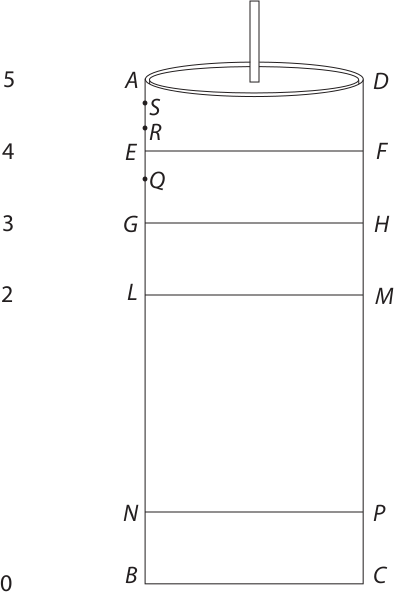
\includegraphics[width=0.43\textwidth]{images/35_5_5v1}\\%\rule[0cm]{2cm}{0cm}
%                \textit{[Fig. 14]}
%                        %\caption{Bildbeschreibung}
%                        \end{center}
%                        %@ @ @ Dies ist eine Abstandszeile - fuer den Fall, dass mehrere figures hintereinander kommen, ohne dass dazwischen laengerer Text steht. Dies kann zu einer Fahlermeldung fuehren. @ @ @ \\
                     \pstart  Praeterea id \edtext{in}{\lemma{}\Afootnote{in \textit{ erg.} \textit{ L}}} quod intrudendum est, seu aer qui recipere debet in spatio \textit{GBCH}, erit ad aerem qui initio recipere debuit in eadem ratione $\rule[-4mm]{0mm}{10mm}\displaystyle \frac{a}{a-2\beta}$. Erit ergo tota difficultas intrudendi aerem spatii \textit{EGHF}, in aerem spatii \textit{GBCH}, \edtext{ad $\delta$, difficultatem}{\lemma{\textit{GBCH},}\Afootnote{ \textit{ (1) }\ ad ratio \textit{ (2) }\ in \textit{ (3) }\ ad $\delta$, difficultatem \textit{ L}}} qua aer \textit{AEFD} intrusus est in aerem \textit{EBCF}, in composita ratione ex ratione $\rule[-4mm]{0mm}{10mm}\displaystyle\frac{a-\beta}{a-2\beta}$, et duplicata $\displaystyle\frac{a}{a-\beta}$, id est ea ratio erit $\rule[-4mm]{0mm}{10mm}\displaystyle \displaystyle \sqcap \frac{a-\beta}{a-2\beta},\smallfrown\frac{a^2}{a-\beta,\square}\sqcap \frac{a^2}{a-\beta, a-2\beta}$ seu difficultas intrudendi aeris \textit{EGHF} in aerem spatii \textit{GBCH}, erit $\rule[-4mm]{0mm}{10mm}\displaystyle \frac{a^2\delta}{a-\beta, a-2\beta}\sqcap\lambda$.
                     \pend 
                     \pstart  Eodem jam modo difficultas computabitur, qua aer \textit{GLMH} intrudendus est in \edtext{aerem}{\lemma{in}\Afootnote{ \textit{ (1) }\ spatium \textit{ (2) }\ aerem \textit{ L}}} \textit{LBCM}. Erit enim ratio difficultatis hujus quam appellabimus \textit{μ}, ad difficultatem $\delta$ in composita ratione ex \edtext{his tribus, quarum reciproca \edtext{\textso{prima}}{\lemma{\textso{prima}}\Afootnote{\textit{doppelt unterstrichen}}} spatiorum recipientium, \textit{LBCM}, \textit{EBCF}, seu ratio $\protect\rule[-4mm]{0mm}{10mm}\displaystyle \frac{EBCF}{LBCM}\sqcap \frac{EB}{LB}\sqcap \frac{a-\beta}{a-3\beta}$; secunda vero et tertia [sunt directae]\edtext{}{\Afootnote{est directa\textit{\ L \"{a}ndert Hrsg. } }} corporum intrudendorum, nempe aeris \textit{GLMH} ad aerem \textit{AEFD}}{\lemma{ex}\Afootnote{ \textit{ (1) }\ reciproca \textso{prima}  \textit{(a)}\ rationum \textit{(b)}\ spatiorum recipientium,  \textit{(aa)}\ \textit{EBCF}, \textit{GBCH}, seu ratione $\displaystyle\frac{GBCH}{EBCF} \sqcap$ \textit{(bb)}\ \textit{LBCM}, \textit{EBCF},  \textit{(aaa)}\ seu ratione  \textit{(aaaa)}\ $\displaystyle \frac{GBCH}{EBCF}\sqcap$ \textit{(bbbb)}\ $\displaystyle \frac{LBCM}{EBCF}\sqcap \frac{LB}{EB}\sqcap$ \textit{(cccc)}\ $\displaystyle \frac{a-3\beta}{a-\beta}$; \textso{secunda} directa corporum intrudendorum, aeris \textit{AEDF} \textit{(bbb)}\  seu ratio $\displaystyle \frac{EBCF}{LBCM}\sqcap \frac{EB}{LB}\sqcap \frac{a-\beta}{a-3\beta}$; secunda vero est directa corporum intrudendorum, nempe aeris \textit{GLMH} ad aerem \textit{AECF} tertia directa corporum recipientium,  \textit{(aaaa)}\ seu aeris \textit{(bbbb)}\ quae aequatur \textit{ (2) }\ his ; [...] \textit{AEFD} \textit{ L}}}
                      et in quae facienda intrusio aeris \textit{LBCM} ad aerem \textit{EBCF} quae duae rationes sunt aequales inter se; \edtext{et eaedem}{\lemma{se;}\Afootnote{ \textit{ (1) }\ aequantur \textit{ (2) }\ reciproca \textit{ (3) }\ et eaedem \textit{ L}}} rationi reciprocae spatiorum \mbox{\textit{GBCH}} et \textit{ABCD}, seu directae: \textit{ABCD} ad \textit{GBCH}, seu \textit{AB} ad [\textit{GB}]\edtext{}{\Afootnote{\textit{LB}\textit{\ L \"{a}ndert Hrsg. } }}, seu \textit{a} ad $a-2\beta$. Ergo ratio $\rule[-4mm]{0mm}{10mm}\displaystyle \frac{\mu}{\delta}$ componitur ex his tribus: $\displaystyle \frac{a-\beta}{a-3\beta}, \frac{a}{a-\beta}, \frac{a}{a-2\beta}$. Jam recollecta ratiocinatione $\rule[-4mm]{0mm}{10mm}\displaystyle \frac{\lambda}{\delta}\sqcap \frac{a-\beta}{a-2\beta}\smallfrown\square\frac{a}{a-\beta}$ et $\displaystyle\frac{\mu}{\delta}\sqcap \frac{a-\beta}{a-3\beta}\smallfrown\square\frac{a}{a-2\beta}$. Et omnes vires, $\lambda$, $\mu$, etc., uno generali nomine appellando \textit{y}, spatia autem \textit{BE}, seu $a-\beta$, et \textit{BG} seu $a-2\beta$, etc., uno generali nomine appellando \textit{x}, et literas hasce variarum sive \edtext{indeterminatarum significationum}{\lemma{sive}\Afootnote{ \textit{ (1) }\ indeterminationum \textit{ (2) }\ indeterminatarum significationum \textit{ L}}} in his aequationibus inventis in locum quantitatum mutabilium substituendo fiet una pro omnibus aequatio duarum indeterminationum, ad quendam locum, $\rule[-4mm]{0mm}{10mm}\displaystyle y\sqcap \frac{a-\beta, a^2, \delta}{x-\beta,,\square,x}$. Et quoniam $\beta$ quantitas infinite parva si ipsi \textit{a} vel \textit{y}, vel \textit{x}, comparetur negligi potest fiet: $\rule[-4mm]{0mm}{10mm}\displaystyle y \sqcap \frac{a^3\delta}{x^3}$, quae est aequatio ad \edtext{Hyperboloeidem}{\lemma{ad}\Afootnote{ \textit{ (1) }\ Hyperbolam \textit{ (2) }\ Hyperboloeidem \textit{ L}}} tertii gradus. Sive vis \edtext{aeris compressi}{\lemma{vis}\Afootnote{ \textit{ (1) }\ Elateri\protect\index{Sachverzeichnis}{elaterium|textit} \textit{ (2) }\ aeris compressi \textit{ L}}} usque ad \textit{E}, erit ad vim aeris compressi\protect\index{Sachverzeichnis}{vis!aeris compressi} usque ad \textit{G}, in ratione rectarum \textit{BE}, \edtext{\textit{BG}, ut reciproca triplicata, seu ut $\displaystyle\frac{1}{BE^3}$ ad $\displaystyle\frac{1}{BG^3}$}{\lemma{\textit{BG},}\Afootnote{ \textit{ (1) }\ reciproca, \textit{ (2) }\ triplicata, seu cum sint ut $\displaystyle\frac{1}{BE^3}$ ad $\displaystyle\frac{1}{BG^3}$ \textit{ (3) }\ ut reciproca triplicata, seu ut $\protect\rule[-4mm]{0mm}{10mm}\displaystyle\frac{1}{BE^3}$ ad $\displaystyle\frac{1}{BG^3}$ \textit{ L}}}, seu ut \edtext{cubus de \textit{BG} ad cubum de \textit{BE}}{\lemma{ut}\Afootnote{ \textit{ (1) }\ \textit{BG}\textsuperscript{3} ad \textit{BE}\textsuperscript{3} seu \textit{u} \textit{ (2) }\ cubus [...] \textit{BE} \textit{ L}}}. \edtext{Hac}{\lemma{\textit{BE}.}\Afootnote{ \textit{ (1) }\ Sed jam video necessario in hac quoque ratiocinatione latere Paralogismum, quia posita \textit{x} $\sqcap$ \textit{a} vis est nulla. Quod hujus tamen calculi vi non contingit. \textit{ (2) }\ Hac \textit{ L}}} demonstratione evincitur falsum \edtext{esse quod initio}{\lemma{esse}\Afootnote{ \textit{ (1) }\ quod semper pro certo habu \textit{ (2) }\ quod initio \textit{ L}}} in mentem \edtext{venerat, scilicet vim}{\lemma{venerat,}\Afootnote{ \textit{ (1) }\ vim \textit{ (2) }\ rationem \textit{ (3) }\ scilicet vim \textit{ L}}} qua aer operculo initio resistit, \edtext{ab \textit{AE} tendenti in \textit{EF}}{\lemma{resistit,}\Afootnote{ \textit{ (1) }\ comprimenti in \textit{A} \textit{ (2) }\ ab \textit{AE} tendenti in \textit{EF} \textit{ L}}}, esse infinite parvam, si vi qua \edtext{aer operculo in puncto quodam distantiae assignabilis ab \textit{A}, ut \textit{N}, prementi, resistit}{\lemma{qua}\Afootnote{ \textit{ (1) }\ aer pergere intellig \textit{ (2) }\ aer [...] resistit \textit{ L}}}, comparetur. Cujus contrarium hoc loco demonstratum est; cum posita \textit{x} linea ordinaria ut \textit{BN}, si scilicet \textit{N} tam ab \textit{A}, quam a \textit{B} spatio assignabili distat; futurum sit, ut \textit{y} seu $\rule[-4mm]{0mm}{10mm}\displaystyle \frac{a^3\delta}{x^3}$ ad $\delta$, seu \textit{a}\textsuperscript{\textit{3}} ad \textit{x}\textsuperscript{3}, rationem habeat assignabilem finitam, triplicatam scilicet rectarum \edtext{assignabilium}{\lemma{rectarum}\Afootnote{ \textit{ (1) }\ assignatarum \textit{ (2) }\ assignabilium \textit{ L}}} \textit{a} et \textit{x}.\pend 
                     \pstart  Porro quae est in quolibet puncto compressionis difficultas, seu resistentia, ea esset vis \edtext{Elaterii,}{\lemma{vis}\Afootnote{ \textit{ (1) }\ aeris \textit{ (2) }\ Elaterii, \textit{ L}}} se restituentis si ablato subito operculo dimitteretur\edtext{. Quod si}{\lemma{dimitteretur}\Afootnote{ \textit{ (1) }\ ; itaque res Elaterii in o \textit{ (2) }\ . Quod si \textit{ L}}} praeterea considerare placeat vim inter restituendum, acceleratione\protect\index{Sachverzeichnis}{acceleratio} quaesitam, nova sane subtilissima orietur \edtext{computatio}{\lemma{orietur}\Afootnote{ \textit{ (1) }\ contemplatio \textit{ (2) }\ computatio \textit{ L}}}, quam adjicere placet. Ponatur ergo operculi obicem \edtext{sive pondus}{\lemma{}\Afootnote{sive pondus \textit{ erg.} \textit{ L}}} auferri in \edtext{\textit{LM}}{\lemma{in}\Afootnote{ \textit{ (1) }\ puncto \textit{ (2) }\ \textit{LM} \textit{ L}}}, rejicietur operculum ab Elaterio\protect\index{Sachverzeichnis}{elaterium}, vi, $\rule[-4mm]{0mm}{10mm}\displaystyle \frac{a^3\delta}{BL^3}$. Ponatur incrementum quod accipit acceleratione\protect\index{Sachverzeichnis}{acceleratio}, dum ab \textit{LM} \edtext{operculum redit}{\lemma{operculum}\Afootnote{ \textit{ (1) }\ transit \textit{ (2) }\ redit \textit{ L}}} ad \textit{GH} per spatium infinite parvum\protect\index{Sachverzeichnis}{spatium!infinite parvum}, esse $\Theta$, erit incrementum \edtext{celeritatis}{\lemma{incrementum}\Afootnote{ \textit{ (1) }\ operculi in \textit{ (2) }\ celeritatis \textit{ L}}}, inter \textit{G} et \textit{E} \edtext{seu $\Psi$}{\lemma{}\Afootnote{seu $\Psi$ \textit{ erg.} \textit{ L}}} ad $\Theta$ incrementum celeritatis\protect\index{Sachverzeichnis}{incrementum!celeritatis} inter \textit{L} et \textit{G} \edtext{in ratione}{\lemma{\textit{G}}\Afootnote{ \textit{ (1) }\ ut re \textit{ (2) }\ in ratione \textit{ L}}} rectarum \textit{LE} et \textit{LG} reciproca \edtext{subduplicata}{\lemma{reciproca}\Afootnote{ \textit{ (1) }\ duplicata \textit{ (2) }\ subduplicata \textit{ L}}} sive 
                     $\rule[-4mm]{0mm}{15mm}\displaystyle \frac{\Psi}{\Theta}\sqcap \frac{\underline{\displaystyle\frac{1}{\surd LE}}}{\displaystyle\frac{1}{\surd LG}}\sqcap\surd\frac{LG}{LE}$ si intelligatur vis Elaterii\protect\index{Sachverzeichnis}{vis!elaterii} se restituentis ubique esse uniformis; per ea quae supra demonstravimus\edtext{. Sed}{\lemma{demonstravimus}\Afootnote{ \textit{ (1) }\ ; incrementum autem quod adjicitur a vi quadam, est ad incrementum quod ab alia vi adjicitur \textit{ (2) }\ . Sed \textit{ L}}} cum vis ipsa continue decrescat difficilis satis et perplexa redditur inquisitio, neque enim satis manifestum est incrementa in virium ratione fore. Res ergo exacte excutienda est.
\pend 
                     \pstart  Ponamus vim Elaterii\protect\index{Sachverzeichnis}{vis!elaterii} se restituentis in \textit{LM} tantam esse, ut \edtext{operculum temporis}{\lemma{ut}\Afootnote{ \textit{ (1) }\ tempore \textit{ (2) }\ operculum temporis \textit{ L}}} quodam \edtext{momento}{\lemma{}\Afootnote{momento \textit{ erg.} \textit{ L}}} $\xi$, percurrat spatium \edtext{infinite parvum}{\lemma{}\Afootnote{infinite parvum \textit{ erg.} \textit{ L}}} $LG \sqcap \beta$\edtext{; acceleratione\protect\index{Sachverzeichnis}{acceleratio} quippe in initio non considerata}{\lemma{$\beta$}\Afootnote{ \textit{ (1) }\ sine acceleratione\protect\index{Sachverzeichnis}{acceleratio|textit}, ut in \textit{i} \textit{ (2) }\ ; acceleratione [...] considerata \textit{ L}}}. \edtext{Secundo autem momento}{\lemma{considerata.}\Afootnote{ \textit{ (1) }\ Dum autem secundum momentum percurrit; praeter vim primam $\displaystyle \frac{a^3\delta}{BL^3}$, accedet vis \textit{ (2) }\ Secundo autem momento \textit{ L}}} priori aequali\edtext{, in cujus initio operculum est in \textit{GH}, movebitur non tantum vi prima, $\protect\rule[-4mm]{0mm}{10mm}\displaystyle \frac{a^3\delta}{BL^3}$, sed et vi, $\displaystyle \frac{a^3\delta}{BG^3}$, eritque spatium \textit{LQ}, quod hoc secundo momento percurret}{\lemma{aequali}\Afootnote{ \textit{ (1) }\ momento, quo \textit{ (2) }\ , in [...] percurret \textit{ L}}}, ad spatium \textit{LG} $\sqcap$ $\beta$ quod percurrit primo, ut $\protect\rule[-4mm]{0mm}{10mm}\displaystyle\frac{a^3\delta}{BL^3}+\frac{a^3\delta}{BG^3}$, ad $\displaystyle \frac{a^3\delta}{BL^3}$, sive erit $\displaystyle LQ\sqcap\beta+\beta \frac{\underline{\displaystyle\frac{a^3\delta}{BG^3}}}{\displaystyle\frac{a^3\delta}{BL^3}}\sqcap\beta+\frac{BL^3\beta}{BG^3}$. Tertio \edtext{ergo}{\lemma{}\Afootnote{ergo \textit{ erg.} \textit{ L}}} temporis momento operculum moveri incipiens ex \textit{Q}, ibi agetur trium virium summa nempe, $\rule[-4mm]{0mm}{10mm}\displaystyle \frac{a^3\delta}{BL^3}+\frac{a^3\delta}{BG^3}+\frac{a^3\delta}{BQ^3\sqcap BL,,+\beta,\smallfrown 1+\displaystyle\frac{BL^3}{BG^3},,, cub.}$ et spatium \textit{QR} temporis momento tertio percursum erit ad spatium $\beta$, ut haec summa ad $\rule[-4mm]{0mm}{10mm}\displaystyle \frac{a^3\delta}{BL^3}$, \edtext{ac}{\lemma{$\displaystyle \frac{a^3\delta}{BL^3}$,}\Afootnote{ \textit{ (1) }\ sive $\beta$ \textit{ (2) }\ ac \textit{ L}}} proinde valor spatii hujus [\textit{LR}]\edtext{}{\Afootnote{\textit{QR}\textit{\ L \"{a}ndert Hrsg. } }}, erit $\rule[-4mm]{0mm}{10mm}\displaystyle \sqcap\hspace{4pt}\beta+\beta\frac{BL^3}{BG^3}+\beta\frac{BL^3}{BL,,+\beta, 1+\displaystyle\frac{BL^3}{BG^3},,, cub.\sqcap BQ^3}$. Quarto temporis momento \edtext{operculum movebitur}{\lemma{momento}\Afootnote{ \textit{ (1) }\ erit \textit{ (2) }\ operculum movebitur \textit{ L}}} summa virium quatuor et spatium [\textit{LS}]\edtext{}{\Afootnote{\textit{RS}\textit{\ L \"{a}ndert Hrsg. } }} eo momento percursum, erit ad spatium$\beta$, ut $\rule[-4mm]{0mm}{10mm}\displaystyle \frac{a^3\delta}{BL^3}+\frac{a^3\delta}{BG^3}+\frac{a^3\delta}{BQ^3}+ \frac{a^3\delta}{BR^3}$, et \textit{RS} erit 
                     $\displaystyle \sqcap\hspace{4pt}\beta + \beta\frac{BL^3}{BG^3}+\beta\frac{BL^3}{BQ^3}+\beta\frac{BL^3}{BR^3}$. \edtext{$\displaystyle BL\sqcap c.$ $LG\sqcap \beta.$ $LQ\sqcap\beta+\beta\displaystyle\frac{c^3}{c+\beta,\boxed{3}}$.}{\lemma{$\displaystyle\beta\frac{BL^3}{BR^3}$}\Afootnote{ \textit{ (1) }\ $BG\sqcap BL + \beta,$ \textit{ (2) }\ $\displaystyle BL\sqcap c.$ $LG\sqcap \beta.$ $LQ\sqcap\beta+\beta\displaystyle\frac{c^3}{c+\beta,\boxed{3}}$ \textit{ L}}}
                     \rule[-4mm]{0mm}{10mm}\edtext{$\displaystyle QR\sqcap\beta+\beta\frac{c^3}{c,+\beta,,\genfrac{}{}{0pt}{}{3}{^\cdotp}}+\beta\frac{c^3}{c,+\beta+\beta\displaystyle\frac{c^3}{c+\beta,\genfrac{}{}{0pt}{}{3}{^\cdotp}},,\genfrac{}{}{0pt}{1}{3}{^\cdotp}}$}
                     {\lemma{$\displaystyle \beta\frac{c^3}{c+\beta, \boxed{3}}$}\Afootnote{ \textit{ (1) }\ $\displaystyle QR\sqcap\beta\smallfrown,\frac{c^3}{c+\beta,^3,}+\frac{c^3}{c}$ \textit{ (2) }\ $\displaystyle QR\sqcap\beta+\beta\frac{c^3}{c,+\beta,,\genfrac{}{}{0pt}{}{3}{^\cdotp}}+\beta \frac{c^3}{c,+\beta+\beta\displaystyle\frac{c^3}{c+\beta,\genfrac{}{}{0pt}{}{3}{^\cdotp}},,\genfrac{}{}{0pt}{}{3}{^\cdotp}}$ \textit{ L}}} $\displaystyle RS \sqcap \beta + \beta\frac{c^3}{c, + \beta,,\genfrac{}{}{0pt}{}{3}{^\cdotp}}+\beta\frac{c^3}{c,+\beta+\beta\displaystyle\frac{c^3}{c,+\beta,,\genfrac{}{}{0pt}{}{3}{^\cdotp}},,\genfrac{}{}{0pt}{1}{3}{^\cdotp}}+\beta\frac{c^3}{c,+\beta+\beta\displaystyle\frac{c^3}{c,+\beta,,\genfrac{}{}{0pt}{}{3}{^\cdotp}}+\displaystyle\frac{c^3}{c,+\beta+\beta\displaystyle\frac{c^3}{c,+\beta,,\genfrac{}{}{0pt}{}{3}{^\cdotp}}},,,}$ quae progressio in infinitum continuata; implebit figuram, quae spatia quolibet \edtext{momento percursa referet}{\lemma{momento}\Afootnote{ \textit{ (1) }\ figuram \textit{ (2) }\ percursa referet \textit{ L}}}. Sed hujusmodi progressionem figura Geometrica includere, quae reapse describi possit, \textit{hoc opus hic labor est}\edtext{}{\lemma{est}\Bfootnote{\textsc{Vergil}, \cite{00246}\textit{Aeneis} VI, 129.}}, cum sit res cui nihil simile tentatum sit a quoquam Geometrarum. Non despero tamen, quod in aliis non ab similibus exemplis res successerit. Caeterum: cum \edtext{}{\lemma{}\Afootnote{cum  \textbar\ data \textit{ gestr.}\ \textbar\ vi, \textit{ L}}}vi, v.g. in \textit{Q}, $\displaystyle a^3\delta,\smallfrown\frac{1}{BL^3}+\frac{1}{BG^3}+\frac{1}{BQ^3}$ \edtext{ponatur $\sqcap$ $\omega$}{\lemma{$\displaystyle \frac{1}{BQ^3}$,}\Afootnote{ \textit{ (1) }\ $\sqcap$ $\omega$ \textit{ (2) }\ detur \textit{ (3) }\ sit \textit{ (4) }\ ponatur $\sqcap$ $\omega$ \textit{ L}}}. Quaerendus est modus ineundi hujus progressionis infinitae $\displaystyle \frac{1}{BL^3}+\frac{1}{BG^3}$ etc. $+ \displaystyle\frac{1}{BQ^3}$ etc. summam, dato termino ultimo, $\displaystyle \frac{1}{BQ^3}$ seu data \textit{BQ}, seu dato spatio et habebitur hoc modo vis. Quod an sit in potestate humana saltem per appropinquationem inquirendum est exactius\edtext{}{\lemma{}\Afootnote{exactius  \textbar\ suo loco \textit{ gestr.}\ \textbar\ . Et \textit{ L}}}. Et vero memini esse partem methodi tangentium inversae. Esto enim figura quaesita \textit{LFI} $\langle$jam$\rangle$ descripta, cujus ordinata aliqua assumta \edtext{\textit{BL}, sequentes \textit{DF}, \textit{KI} etc. differentiae \textit{EF}, \textit{HI} etc.}{\lemma{assumta}\Afootnote{ \textit{ (1) }\ \textit{BC} repraesentet, rectam \textit{BL}, et \textit{DF} rectam \textit{BQ} et \textit{KI} rectam \textit{BR} etc. at \textit{BD}. \textit{DK} $\langle$inter$\rangle$ $\langle$--$\rangle$ et \textit{EF}, \textit{HI} spatia \textit{LQ}, \textit{QR} etc. addatur. Caeterum \textit{ (2) }\ \textit{BL}, [...] etc. \textit{ L}}}
                     \pend 
%  Zeitz auskommentiert                       \begin{center}                    
%                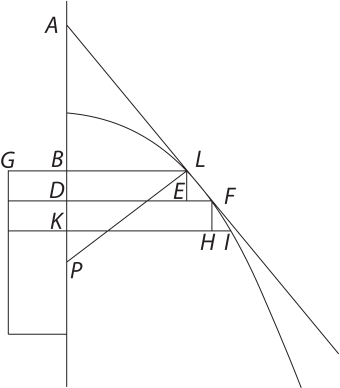
\includegraphics[width=0.45\textwidth]{images/35_5_5v2}\\\textit{[Fig. 15]}
%                        %\caption{Bildbeschreibung}
%                        \end{center}
%                        %@ @ @ Dies ist eine Abstandszeile - fuer den Fall, dass mehrere figures hintereinander kommen, ohne dass dazwischen laengerer Text steht. Dies kann zu einer Fahlermeldung fuehren. @ @ @ \\

                     \pstart  Unde calculus talis\footnote{\textit{Am linken Rand quer}: \textso{Demonstratio accurata} quae vero tribus paginis praecedentibus continentur lapsibus plena sunt quorum origines ibi in margine notavi. \textit{Darunter}: Vide haec pertinentia clarius Schediasmata de progressionibus et geometria arcana Xb 1674.% @@@Hier fehlt noch eine Bfootnote(1674.: Vgl. \cite{00261}\textit{LSB} VII, 3 N. 39.)
                     }
                     \edtext{}{\lemma{1674}\linenum{|15|||15|}\Bfootnote{Vgl. \cite{00261}\textit{LSB} VII, 3 N. 39.}} qualem jam subjiciam ponendo \edtext{primam ordinatarum}{\lemma{}\Afootnote{primam ordinatarum \textit{ erg.} \textit{ L}}} \textit{BL} et \textit{LE}  \edtext{intervallum seu \textit{BD}}{\lemma{}\Afootnote{intervallum seu \textit{BD} \textit{ erg.} \textit{ L}}}, et \textit{AB} productam axis tangenti \textit{AL} occurrentem esse 
                                    datos, unde sequentes quaerantur; \edtext{ponamus}{\lemma{quaerantur;}\Afootnote{ \textit{ (1) }\ fiet eni \textit{ (2) }\ nam \textit{ (3) }\ ponamus \textit{ L}}} \edtext{productam}{\lemma{ponamus}\Afootnote{ \textit{ (1) }\ tangentem \textit{ (2) }\ productam \textit{ L}}} \textit{AB} vel \textit{AD}, etc. $\sqcap \hspace{4pt}l$. erit $\displaystyle EF \sqcap BL,\smallfrown\frac{EL}{l}$ atque ita continuando calculum ad sequentes quoque ordinatas inveniendas, fiet calculus in se replicatus similis proposito, qui si conferantur, patebit. Ponendo ordinatam $\sqcap$ \textit{y}, esse $l \sqcap y^4$, nam dividens \textit{y}, relinquit $\displaystyle\frac{1}{y^3}$ \edtext{itaque}{\lemma{$\displaystyle\frac{1}{y^3}$}\Afootnote{ \textit{ (1) }\ quia \textit{ (2) }\ itaque \textit{ L}}} $\displaystyle \frac{y}{l}\sqcap \frac{1}{y^3}$. Ergo  $l \sqcap y^4$. Jam alibi $\displaystyle l \sqcap \frac{y^2}{p}$. Ponendo \textit{p} $\sqcap$ reductae seu interceptae inter perpendicularem et ordinatam, fiet $\displaystyle p\sqcap \frac{1}{y}\sqcap BP$. Calculus: $\displaystyle LE \sqcap\beta$. $BL\sqcap c$.  $DF \sqcap BL+EF$. $\displaystyle EF \sqcap BL, \smallfrown \frac{LE}{AB}$. Ergo [$\displaystyle DF \sqcap DE \sqcap c + \frac{c \smallfrown\beta}{l}$]\edtext{}{\lemma{
                   $\displaystyle DF \sqcap BE \sqcap c + \frac{c \smallfrown\beta}{l}$
                   }\Afootnote{ \textit{\ L \"{a}ndert Hrsg.}}} \edtext{. Et [$\displaystyle KI \sqcap c + \frac{c\beta}{l}+\frac{c+\displaystyle\frac{c\beta}{l}}{(l)}$]\edtext{}{\lemma{$\displaystyle GI \sqcap c + \frac{c\beta}{l}+\frac{c+\displaystyle\frac{c\beta}{l}}{(l)}$]}\Afootnote{ \textit{\ L \"{a}ndert Hrsg.}}}}{\lemma{$\displaystyle \frac{c \smallfrown\beta}{l}$]}\Afootnote{ \textit{ (1) }\ et $\displaystyle GI \sqcap c + \frac{c\beta}{l}+ \frac{c\beta}{c+\displaystyle\frac{c\beta}{l}}$ \textit{ (2) }\ . Et [$\displaystyle KI \sqcap c + \frac{c\beta}{l}+\frac{c+\displaystyle\frac{c\beta}{l}}{(l)}$] \textit{ L}}}. Ipsis ergo 
                     \edtext{[\textit{BL}, \textit{DF}, \textit{KI}]\edtext{}{\Afootnote{\textit{BC}, \textit{DF}, \textit{GI}\textit{\ L \"{a}ndert Hrsg. } }}, repraesentabuntur spatia \textit{BG}, \textit{BQ}, \textit{BR}}{\lemma{ergo}\Afootnote{ \textit{ (1) }\ \textit{GI} repraesentabuntur spatia, \textit{B} \textit{ (2) }\ [\textit{BL}, \textit{DF}, \textit{KI}], repraesentabuntur spatia  \textbar\ percursa \textit{ gestr.}\ \textbar\  \textit{BG}, \textit{BQ}, \textit{BR} \textit{ L}}},\rule[-1cm]{0cm}{0cm} et posita \textit{DF} $\sqcap$ \textit{y} erit $ l \sqcap y^2$ et fiet: jam $\displaystyle l \sqcap \frac{y^2}{p}$ ergo $\displaystyle \frac{y^2}{p}\sqcap y^3,$ sive $\displaystyle \frac{1}{p}\sqcap y$. Quaerenda ergo figura in qua \edtext{reductae sint}{\lemma{qua}\Afootnote{ \textit{ (1) }\ productae \textit{ (2) }\ productae sint \textit{ (3) }\ reductae sint \textit{ L}}} ordinatis reciproce proportionales quae erit quaesita.\footnote{
                 %    \pstart
                 \textit{Nebenrechnung am linken Rand von Bl. 6 r\textsuperscript{o} ohne Beziehung zum Text:} \newline$\protect\begin{array}{r}3\\\protect\underline{15}\\45\\\protect\underline{30}\\75\\\protect\underline{10}\\\protect\underline{85}\protect\end{array}$}
                 \pend 